%beamer

% Define a global usable date. Must come before StyleTut
% \newcommand{\mydate}{11.11.2016}

% Comment/uncomment this line to toggle handout mode
% \newcommand{\handout}{}

%% Beamer-Klasse im korrekten Modus
\ifdefined \handout
\documentclass[handout]{beamer} % Handout mode
\else
\documentclass{beamer}
\fi

%% UTF-8-Encoding
\usepackage[utf8]{inputenc}

% % \bigtimes abgeschrieben von http://tex.stackexchange.com/questions/14386/importing-a-single-symbol-from-a-different-font
% \DeclareFontFamily{U}{mathx}{\hyphenchar\font45}
% \DeclareFontShape{U}{mathx}{m}{n}{
%       <5> <6> <7> <8> <9> <10> gen * mathx
%       <10.95> mathx10 <12> <14.4> <17.28> <20.74> <24.88> mathx12
%       }{}
% \DeclareSymbolFont{mathx}{U}{mathx}{m}{n}
% \DeclareMathSymbol{\bigtimes}{\mathop}{mathx}{161}

\RequirePackage{xcolor}

\def\9{\square}
%\def\9{\blank}

% f"ur Aussagenlogik
\colorlet{alcolor}{blue}
\RequirePackage{tikz}
\usetikzlibrary{arrows.meta}
\newcommand{\alimpl}{\mathrel{\tikz[x={(0.1ex,0ex)},y={(0ex,0.1ex)},>={Classical TikZ Rightarrow[]}]{\draw[alcolor,->,line width=0.7pt,line cap=round] (0,0) -- (15,0);\path (0,-6);}}}
\newcommand{\aleqv}{\mathrel{\tikz[x={(0.1ex,0ex)},y={(0ex,0.1ex)},>={Classical TikZ Rightarrow[]}]{\draw[alcolor,<->,line width=0.7pt,line cap=round] (0,0) -- (18,0);\path (0,-6);}}}
\newcommand{\aland}{\mathbin{\raisebox{-0.6pt}{\rotatebox{90}{\texttt{\color{alcolor}\char62}}}}}
\newcommand{\alor}{\mathbin{\raisebox{-0.8pt}{\rotatebox{90}{\texttt{\color{alcolor}\char60}}}}}
%\newcommand{\ali}[1]{_{\mathtt{\color{alcolor}#1}}}
\newcommand{\alv}[1]{\mathtt{\color{alcolor}#1}}
\newcommand{\alnot}{\mathop{\tikz[x={(0.1ex,0ex)},y={(0ex,0.1ex)}]{\draw[alcolor,line width=0.7pt,line cap=round,line join=round] (0,0) -- (10,0) -- (10,-4);\path (0,-8) ;}}}
\newcommand{\alP}{\alv{P}} %ali{#1}}
%\newcommand{\alka}{\negthinspace\hbox{\texttt{\color{alcolor}(}}}
\newcommand{\alka}{\negthinspace\text{\texttt{\color{alcolor}(}}}
%\newcommand{\alkz}{\texttt{\color{alcolor})}}\negthinspace}
\newcommand{\alkz}{\text{\texttt{\color{alcolor})}}\negthinspace}
\newcommand{\AAL}{A_{AL}}
\newcommand{\LAL}{\hbox{\textit{For}}_{AL}}
\newcommand{\AxAL}{\hbox{\textit{Ax}}_{AL}}
\newcommand{\AxEq}{\hbox{\textit{Ax}}_{Eq}}
\newcommand{\AxPL}{\hbox{\textit{Ax}}_{PL}}
\newcommand{\AALV}{\hbox{\textit{Var}}_{AL}}
\newcommand{\MP}{\hbox{\textit{MP}}}
\newcommand{\GEN}{\hbox{\textit{GEN}}}
\newcommand{\W}{\ensuremath{\hbox{\textbf{w}}}\xspace}
\newcommand{\F}{\ensuremath{\hbox{\textbf{f}}}\xspace}
\newcommand{\WF}{\ensuremath{\{\W,\F\}}\xspace}
\newcommand{\val}{\hbox{\textit{val}}}
\newcommand{\valDIb}{\val_{D,I,\beta}}

\newcommand*{\from}{\colon}

% die nachfolgenden Sachen angepasst an cmtt
\newlength{\ttquantwd}
\setlength{\ttquantwd}{1ex}
\newlength{\ttquantht}
\setlength{\ttquantht}{6.75pt}
\def\plall{%
  \tikz[line width=0.67pt,line cap=round,line join=round,baseline=(B),alcolor] {
    \draw (-0.5\ttquantwd,\ttquantht) -- node[coordinate,pos=0.4] (lll){} (-0.25pt,-0.0pt) -- (0.25pt,-0.0pt) -- node[coordinate,pos=0.6] (rrr){} (0.5\ttquantwd,\ttquantht);
    \draw (lll) -- (rrr);
    \coordinate (B) at (0,-0.35pt);
  }%
}
\def\plexist{%
  \tikz[line width=0.67pt,line cap=round,line join=round,baseline=(B),alcolor] {
    \draw (-0.9\ttquantwd,\ttquantht) -- (0,\ttquantht) -- node[coordinate,pos=0.5] (mmm){} (0,0) --  (-0.9\ttquantwd,0);
    \draw (mmm) -- ++(-0.75\ttquantwd,0);
    \coordinate (B) at (0,-0.35pt);
  }\ensuremath{\,}%
}
\let\plexists=\plexist
\newcommand{\NT}[1]{\ensuremath{\langle\mathrm{#1} \rangle}}

\newcommand{\CPL}{\text{\itshape Const}_{PL}}
\newcommand{\FPL}{\text{\itshape Fun}_{PL}}
\newcommand{\RPL}{\text{\itshape Rel}_{PL}}
\newcommand{\VPL}{\text{\itshape Var}_{PL}}
\newcommand{\ATer}{A_{\text{\itshape Ter}}}
\newcommand{\ARel}{A_{\text{\itshape Rel}}}
\newcommand{\AFor}{A_{\text{\itshape For}}}
\newcommand{\LTer}{L_{\text{\itshape Ter}}}
\newcommand{\LRel}{L_{\text{\itshape Rel}}}
\newcommand{\LFor}{L_{\text{\itshape For}}}
\newcommand{\NTer}{N_{\text{\itshape Ter}}}
\newcommand{\NRel}{N_{\text{\itshape Rel}}}
\newcommand{\NFor}{N_{\text{\itshape For}}}
\newcommand{\PTer}{P_{\text{\itshape Ter}}}
\newcommand{\PRel}{P_{\text{\itshape Rel}}}
\newcommand{\PFor}{P_{\text{\itshape For}}}

\newcommand{\plka}{\alka}
\newcommand{\plkz}{\alkz}
%\newcommand{\plka}{\plfoo{(}}
%\newcommand{\plkz}{\plfoo{)}}
\newcommand{\plcomma}{\hbox{\texttt{\color{alcolor},}}}
\newcommand{\pleq}{{\color{alcolor}\,\dot=\,}}

% MODIFIED (DJ)
% previously: \newcommand{\plfoo}[1]{\mathtt{\color{alcolor}#1}}
\newcommand{\plfoo}[1]{\texttt{\color{alcolor}#1}}

\newcommand{\plc}{\plfoo{c}}
\newcommand{\pld}{\plfoo{d}}
\newcommand{\plf}{\plfoo{f}}
\newcommand{\plg}{\plfoo{g}}
\newcommand{\plh}{\plfoo{h}}
\newcommand{\plx}{\plfoo{x}}
\newcommand{\ply}{\plfoo{y}}
\newcommand{\plz}{\plfoo{z}}
\newcommand{\plR}{\plfoo{R}}
\newcommand{\plS}{\plfoo{S}}

\newcommand{\bv}{\mathrm{bv}}
\newcommand{\fv}{\mathrm{fv}}

%\newcommand{\AxAL}{\hbox{\textit{Ax}}_{AL}}
%\newcommand{\AALV}{\hbox{\textit{Var}}_{AL}}

%\renewcommand{\#}[1]{\literal{#1}}
\newcommand{\A}{\mathcal{A}}
\newcommand{\Adr}{\text{Adr}}
\newcommand{\ar}{\mathrm{ar}}
\newcommand{\ascii}[1]{\literal{\char#1}}
%\newcommand{\assert}[1]{\text{/\!\!/\ } #1}
\newcommand{\assert}[1]{\colorbox{black!7!white}{\ensuremath{\{\;#1\;\}}}}
\newcommand{\Assert}[1]{$\langle$\textit{#1}$\rangle$}
\newcommand{\B}{\mathcal{B}}
\newcommand{\bfmod}{\mathbin{\kw{ mod }}}
\newcommand{\bb}{{\text{bb}}}
\def\bottom{\hbox{\small$\pmb{\bot}$}}
\newcommand{\card}[1]{|#1|}
%\newcommand{\cod}{\mathop{\text{cod}}}  % ist in thwmathabbrevs
\newcommand{\Conf}{\mathcal{C}}
\newcommand{\define}[1]{\emph{#1}}
%\renewcommand{\dh}{d.\,h.\@\xspace}
%\newcommand{\Dh}{D.\,h.\@\xspace}
%\newcommand{\engl}[1]{engl.\xspace\emph{#1}}
\newcommand{\eps}{\varepsilon}
%\newcommand{\evtl}{evtl.\@\xspace}
\newcommand{\fbin}{\text{bin}}
\newcommand{\finv}{\text{inv}}
\newcommand{\fnum}{\text{num}}
\newcommand{\fNum}{{\text{Num}}}
\newcommand{\frepr}{\text{repr}}
\newcommand{\fRepr}{\text{Repr}}
\newcommand{\fZkpl}{\text{Zkpl}}
\newcommand{\fLen}{\text{Len}}
\newcommand{\fsem}{\text{sem}}
\providecommand{\fspace}{\mathord{\text{space}}}
\providecommand{\fSpace}{\mathord{\text{Space}}}
\providecommand{\ftime}{\mathord{\text{time}}}
\providecommand{\fTime}{\mathord{\text{Time}}}
\newcommand{\fTrans}{\text{Trans}}
\newcommand{\fVal}{\text{Val}}

% Modified (DJ)
\newcommand{\Val}{\text{Val}}

%\def\G{\mathbb{Z}}
\newcommand{\HT}[1]{\normalfont\textsc{HT-#1}}
\newcommand{\htr}[3]{\{#1\}\;#2\; \{#3\}}
\newcommand{\Id}{\text{I}}
%\newcommand{\ie}{i.\,e.\@\xspace}
\newcommand{\instr}[2]{\texttt{#1}\ \textit{#2}}
\newcommand{\Instr}[2]{\texttt{#1}\ \textrm{#2}}
\newcommand{\instrr}[3]{\texttt{#1}\ \textit{#2}\texttt{(#3)}}
\newcommand{\Instrr}[3]{\texttt{#1}\ \textrm{#2}\texttt{(#3)}}
\newcommand{\io}{\!\mid\!}
\usepackage{KITcolors}
\newcommand{\literal}[1]{\hbox{\textcolor{blue!95!white}{\textup{\texttt{\scalebox{1.11}{#1}}}}}}
%\newcommand{\literal}[1]{\hbox{\textcolor{KITblue!80!black}{\textup{\texttt{#1}}}}}
\def\kasten#1{\leavevmode\literal{\setlength{\fboxsep}{1pt}\fbox{\vrule  width 0pt height 1.5ex depth 0.5ex #1}}}
\newcommand{\kw}[1]{\ensuremath{\mathbf{#1}}}
\newcommand{\lang}[1]{\ensuremath{\langle#1\rangle}}
%\newcommand{\maw}{m.\,a.\,w.\@\xspace}
%\newcommand{\MaW}{M.\,a.\,w.\@\xspace}
\newcommand{\mdefine}[2][FOOBAR]{\define{#2}\def\foobar{FOOBAR}\def\optarg{#1}\ifx\foobar\optarg\def\optarg{#2}\fi\graffito{\optarg}}
\newcommand{\meins}{\rotatebox[origin=c]{180}{1}}
\newcommand{\Mem}{\text{Mem}}
\newcommand{\memread}{\text{memread}}
\newcommand{\memwrite}{\text{memwrite}}
\providecommand{\meta}[1]{\ensuremath{\langle}\textit{#1}\ensuremath{\rangle}}
%\newcommand{\N}{\mathbb{N}}
\newcommand{\NP}{\mathbf{NP}}
\newcommand{\Nadd}{N_{\text{add}}}
\newcommand{\Nmult}{N_{\text{mult}}}
\newcommand{\Oh}[1]{O\left(#1\right)}
\newcommand{\Om}[1]{\Omega\left(#1\right)}
\newcommand{\personname}[1]{\textsc{#1}}
\newcommand{\regname}[1]{\texttt{#1}}
\newcommand{\mima}{\textsc{Mima}\xspace}
\newcommand{\mimax}{\textsc{Mima-X}\xspace}

\def\Pclass{\text{\bfseries P}}
\def\PSPACE{\text{\bfseries PSPACE}}

\newcommand{\SPush}{\text{push}}
\newcommand{\SPop}{\text{pop}}
\newcommand{\SPeek}{\text{peek}}
\newcommand{\STop}{\text{top}}
\newcommand{\STos}{\text{\itshape tos}}
\newcommand{\SBos}{\text{\itshape bos}}

%\newcommand{\R}{\mathbb{R}}
\newcommand{\Rnullplus}{\R_0^{+}}
\newcommand{\Rplus}{\R_{+}}
\newcommand{\resp}{resp.\@\xspace}
\newcommand{\Sem}{\text{Sem}}
\newcommand{\sgn}{\mathop{\text{sgn}}}
\newcommand{\sqbox}{\mathop{\raisebox{-6.2pt}{\hbox{\hbox to 0pt{$^{^{\sqcap}}$\hss}$^{^{\sqcup}}$}}}}
\newcommand{\sqleq}{\sqsubseteq}
\newcommand{\sqgeq}{\sqsupseteq}
\newcommand{\Th}[1]{\Theta\left(#1\right)}
%\newcommand{\usw}{usw.\@\xspace}
\newcommand{\V}[1]{\hbox{\textit{#1}}}
\newcommand{\x}{\times}
\newcommand{\ZK}{\mathbb{K}}
%\newcommand{\Z}{\mathbb{Z}}
%\newcommand{\zB}{z.\,B.\@\xspace}
%\newcommand{\ZB}{Z.\,B.\@\xspace}
% \newcommand{\bb}{{\text{bb}}}
% \def\##1{\hbox{\textcolor{darkblue}{\texttt{#1}}}}
% \def\A{\mathcal{A}}
% \newcommand{\0}{\#0}
% \newcommand{\1}{\#1}
% \newcommand{\Obj}{\text{Obj}}
% \newcommand{\start}{\mathop{\text{start}}}
% \newcommand{\compactlist}{\addtolength{\itemsep}{-\parskip}}
% \newcommand{\fval}{\text{val}}
% \newcommand{\lang}[1]{\ensuremath{\langle#1\rangle}}
% \newcommand{\io}{\!\mid\!}
% \def\sqbox{\mathop{\raisebox{-6.2pt}{\hbox{\hbox to 0pt{$^{^{\sqcap}}$\hss}$^{^{\sqcup}}$}}}}
% \def\sqleq{\sqsubseteq}
% \def\sqgeq{\sqsupseteq}
\def\Td{T_{\overline{d}}}
% \newcommand{\csym}[1]{\ensuremath{\#{c}_{\#{\hbox{\scriptsize #1}}}}}
% \newcommand{\F}{\ensuremath{\mathcal{F}}}
% \newcommand{\fsym}[2]{\ensuremath{\#{f}^{\#{\hbox{\scriptsize #1}}}_{\#{\hbox{\scriptsize #2}}}}}
% \newcommand{\rsym}[2]{\ensuremath{\#{R}^{\#{\hbox{\scriptsize #1}}}_{\#{\hbox{\scriptsize #2}}}}}
% \newcommand{\xsym}[1]{\ensuremath{\#{x}_{\#{\hbox{\scriptsize #1}}}}}
% \newcommand{\I}{\mathcal{I}}
% ********************************************************************

\usepackage{../TutTexbib/thwregex}
\usepackage{environ}
\usepackage{bm}
\usepackage{calc}
\usepackage{varwidth}
\usepackage{wasysym}
\usepackage{mathtools}

%% Tabellen
\usepackage{array}
\usepackage{multicol}

%% Bibliotheken für viele mathematische Symbole
\usepackage{amsmath, amsfonts, amssymb}



% This is a configuration file with personal tutor information.
% It is therefore excluded from the git repository, so changes in this file will not conflict in git commits.

% Copy this template, rename to config.tex and add your information below.

\newcommand{\myname}{Lukas Morawietz}
\newcommand{\mymail}{lukas.morawietz@gmail.com} % Consider using your named student mail address to keep your u**** account private.
\newcommand{\mytutnumber}{31}

% Don't forget to update ILIAS url. WARNING: Underscores '_' and Ampersands '&' have to be escaped with backslashes '\'. Blame TeX, not me.
\newcommand{\myILIASurl}{https://ilias.studium.kit.edu/ilias.php?ref\_id=855240\&cmdClass=ilrepositorygui\&cmdNode=5r\&baseClass=ilrepositorygui}

% Uncommenting this will print Socrative info with here defined roomname whenever \Socrative is called.
% (Otherwise, \Socrative will remain silent.)
% \newcommand{\mysocrativeroom}{???}

%\def\ThassesTut{}
\def\DanielsTut{}

\newcommand{\aboutMeFrame}{
	\begin{frame}{Über mich}
		\myname \\
		Informatik, 9. Fachsemester (Bachelor)
		% Lebensgeschichte...
		% Stammbaum...
		% Aufarbeitung der eigenen Todesser-Vergangenheit...
	\end{frame}
}

\def\thisyear{2019}

% Update date of exam
\def\myKlausurtermin{18.~März~2020, 14:00–16:00~Uhr}

\def\mydate#1{
		  \ifnum#1=1\relax	  23. Oktober \thisyear \
	\else \ifnum#1=2\relax	  30. Oktober \thisyear \
	\else \ifnum#1=3\relax    06. November \thisyear \
	\else \ifnum#1=4\relax    13. November \thisyear \
	\else \ifnum#1=5\relax    20. November \thisyear \
	\else \ifnum#1=6\relax    27. November \thisyear \
	\else \ifnum#1=7\relax    04. Dezember \thisyear \
	\else \ifnum#1=8\relax    11. Dezember \thisyear \
	\else \ifnum#1=9\relax    18. Dezember \thisyear \
	\else \ifnum#1=10\relax   08. Januar \nextyear \
	\else \ifnum#1=11\relax   15. Januar \nextyear \
	\else \ifnum#1=12\relax   22. Januar \nextyear \
	\else \ifnum#1=13\relax   29. Januar \nextyear \
	\else \ifnum#1=14\relax   05. Februar \nextyear \
	\else \textbf{Datum undefiniert!} 
	\fi\fi\fi\fi\fi\fi\fi\fi\fi\fi\fi\fi\fi\fi
}

\def\mylasttimestext{Was letztes Mal geschah...}

\colorlet{beamerlightred}{red!40}
\colorlet{beamerlightgreen}{green!50}
\colorlet{beamerlightyellow}{yellow!50}
\colorlet{lightred}{red!30}
\colorlet{lightgreen}{green!40}
\colorlet{lightyellow}{yellow!50}
\colorlet{fullred}{red!60}
\colorlet{fullgreen}{green}

\definecolor{myalertcolor}{rgb}{1,0.33,0.24}
\setbeamercolor{alerted text}{fg=myalertcolor}

% Flag to toggle display of KIT Logo.
% If you want to conform to the official logo guidelines, 
% you are not allowed to use the logo and should disable it
% using the following flag. Just saying.
% (But it's too beautiful, so best leave this commented. :P)
%\newcommand{\noKITLogo}{}

% Toggle handout mode by including the following line before including PraeambelTut
% and removing the % at the start (but do NOT remove the % char here, otherwise handout mode will always be on!)
% Please keep handout mode off in all commits!

% \newcommand{\handout}{}



% define custom \handout command flag if handout mode is toggled  #DirtyAsHellButWell...
\only<beamer:0>{\def\handout{}} %beamer:0 == handout mode

\newcommand{\R}{\mathbb{R}}
\newcommand{\N}{\mathbb{N}}
\newcommand{\Z}{\mathbb{Z}}
\newcommand{\Q}{\mathbb{Q}}
\newcommand{\BB}{\mathbb{B}}
\newcommand{\C}{\mathbb{C}}
\newcommand{\K}{\mathbb{K}}
\newcommand{\G}{\mathbb{G}}
\newcommand{\nullel}{\mathcal{O}}
\newcommand{\einsel}{\mathds{1}}
\newcommand{\Pot}{\mathcal{P}}
\renewcommand{\O}{\text{O}}

\def\word#1{\hbox{\textcolor{blue}{\texttt{#1}}}}
\let\literal\word
\def\mword#1{\hbox{\textcolor{blue}{$\mathtt{#1}$}}}  % math word
\def\sp{\scalebox{1}[.5]{\textvisiblespace}}
\def\wordsp{\word{\sp}}

%\newcommand{\literal}[1]{\textcolor{blue}{\texttt{#1}}}
\newcommand{\realTilde}{\textasciitilde \ }
\newcommand{\setsize}[1]{\ensuremath{\left\lvert #1 \right\rvert}}
\let\size\setsize
\newcommand{\set}[1]{\left\{#1\right\}}
\newcommand{\tuple}[1]{\left(#1\right)}
\newcommand{\normalvar}[1]{\text{$#1$}}

% Modified by DJ
\let\oldemptyset\emptyset
\let\emptyset\varnothing % proper emptyset

%\definecolor{myRed}{RGB}{255,75,20}
%\colorlet{myGreen}{KITpalegreen}

%\newcounter{tfqtempcount}
%\newcommand{\truefalseQ}[4]{
%	\setcounter{tfqtempcount}{#1}
%	\addtocounter{tfqtempcount}{1}
%	\truefalseQuestion{#1}{\value{tfqtempcount}}{#2}{#3}{#4}
%}

%\newcommand{\truefalseQuestion}[5]{\item<#1-|handout:#1-> \color<#2-|handout:#2->{#3} #4 \qquad \visible<#2-|handout:#2->{#5}}

\newcommand{\boder}{\ensuremath{\mathbin{\textcolor{blue}{\vee}}}\xspace}
\newcommand{\bund}{\ensuremath{\mathbin{\textcolor{blue}{\wedge}}}\xspace}
\newcommand{\bimp}{\ensuremath{\mathrel{\textcolor{blue}{\to}}}\xspace}
\newcommand{\bgdw}{\ensuremath{\mathrel{\textcolor{blue}{\leftrightarrow}}}\xspace}
\newcommand{\bnot}{\ensuremath{\textcolor{blue}{\neg}}\xspace}
\newcommand{\bone}{\ensuremath{\textcolor{blue}{1}}\text{}}
\newcommand{\bzero}{\ensuremath{\textcolor{blue}{0}}\text{}}
\newcommand{\bleftBr}{\ensuremath{\textcolor{blue}{\texttt{(}}}\text{}}
\newcommand{\brightBr}{\ensuremath{\textcolor{blue}{\texttt{)}}}\text{}}

\newcommand{\plB}{\plfoo{B}}
\newcommand{\plE}{\plfoo{E}}

\newcommand{\summe}[2]{\sum\limits_{#1}^{#2}}
\newcommand{\limes}[1]{\lim\limits_{#1}}

%\newcommand{\numpp}{\advance \value{weeknum} by -2 \theweeknum \advance \value{weeknum} by 2}
%\newcommand{\nump}{\advance \value{weeknum} by -1 \theweeknum \advance \value{weeknum} by 1}

\newcommand{\mycomment}[1]{}
\newcommand{\Comment}[1]{}

%% DISCLAIMER START 
% It is INSANELY IMPORTANT NOT TO DO THIS OUTSIDE BEAMER CLASS! IN ARTCILE DOCUMENTS, THIS IS VERY LIKELY TO BUG AROUND!
\makeatletter%
\@ifclassloaded{beamer}%
{
	% TODO 
	% no time...
	% redefine section to ignore multiple \section calls with the same title
}%
{
	\errmessage{ERROR: section command redefinition outside of beamer class document! Please contact the author of this code.}
}%
\makeatother%
%% DISCLAIMER END

\newcounter{abc}
\newenvironment{alist}{
  \begin{list}{(\alph{abc})}{
      \usecounter{abc}\setlength{\leftmargin}{8mm}\setlength{\labelsep}{2mm}
    }
}{\end{list}}


\newcommand{\stdarraystretch}{1.20}
\renewcommand{\arraystretch}{\stdarraystretch}  % for proper row spacing in tables

\newcommand{\morescalingdelimiters}{   % for proper \left( \right) typography
	\delimitershortfall=-1pt  
	\delimiterfactor=1
}

\newcommand{\centered}[1]{\vspace{-\baselineskip}\begin{center}#1\end{center}\vspace{-\baselineskip}}

% for \implitem and \item[bla] stuff to look right:
\setbeamercolor*{itemize item}{fg=black}
\setbeamercolor*{itemize subitem}{fg=black}
\setbeamercolor*{itemize subsubitem}{fg=black}

\setbeamercolor*{description item}{fg=black}
\setbeamercolor*{description subitem}{fg=black}
\setbeamercolor*{description subsubitem}{fg=black}

\renewcommand{\qedsymbol}{\textcolor{black}{\openbox}}

\renewcommand{\mod}{\mathop{\textbf{mod}}}
\renewcommand{\div}{\mathop{\textbf{div}}}

\newcommand{\ceil}[1]{\left\lceil#1\right\rceil}
\newcommand{\floor}[1]{\left\lfloor#1\right\rfloor}
\newcommand{\abs}[1]{\left\lvert #1 \right\rvert}
\newcommand{\Matrix}[1]{\begin{pmatrix} #1 \end{pmatrix}}
\newcommand{\braced}[1]{\left\lbrace #1 \right\rbrace}

\def\fract#1/#2 {\frac{#1}{#2}} % ! Trailing space is crucial!
\def\dfract#1/#2 {\dfrac{#1}{#2}} % ! Trailing space is crucial!

\newcommand{\Mid}{\;\middle|\;}

\let\after\circ

\def\·{\cdot}
\def\*{\cdot}
\def\?>{\ensuremath{\rightsquigarrow}}  % Fuck you, Latex

\newcommand{\tight}[1]{{\renewcommand{\arraystretch}{0.76} #1}}
\newcommand{\stackedtight}[1]{{\renewcommand{\arraystretch}{0.76} \begin{matrix} #1 \end{matrix}} }
\newcommand{\stacked}[1]{\begin{matrix} #1 \end{matrix} }
\newcommand{\casesl}[1]{\delimitershortfall=0pt  \left\lbrace\hspace{-.3\baselineskip}\begin{array}{ll} #1 \end{array}\right.}
\newcommand{\casesr}[1]{\delimitershortfall=0pt  \left.\begin{array}{ll} #1 \end{array}\hspace{-.3\baselineskip}\right\rbrace}
\newcommand{\caseslr}[1]{\delimitershortfall=0pt  \left\lbrace\hspace{-.3\baselineskip}\begin{array}{ll} #1 \end{array}\hspace{-.3\baselineskip}\right\rbrace}

\def\q#1uad{\ifnum#1=0\relax\else\quad\q{\the\numexpr#1-1\relax}uad\fi}
% e.g. \q1uad = \quad, \q2uad = \qquad etc.

\newcommand{\qqquad}{\q3uad}

\newcommand{\impl}{\ifmmode\ensuremath{\mskip\thinmuskip\Rightarrow\mskip\thinmuskip}\else$\Rightarrow$\fi\xspace}
\newcommand{\Impl}{\ifmmode\implies\else$\Longrightarrow$\fi\xspace}

\newcommand{\derives}{\Rightarrow}

\newcommand{\gdw}{\ifmmode\mskip\thickmuskip\Leftrightarrow\mskip\thickmuskip\else$\Leftrightarrow$\fi\xspace}
\newcommand{\Gdw}{\ifmmode\iff\else$\Longleftrightarrow$\fi\xspace}

\newcommand{\symbitemnegoffset}{\hspace{-.5\baselineskip}}
\newcommand{\implitem}{\item[\impl\symbitemnegoffset]}
\newcommand{\Implitem}{\item[\Impl\symbitemnegoffset]}


\newcommand{\forcenewline}{\mbox{}\\}


% proper math typography
\newcommand{\functionto}{\longrightarrow}
\renewcommand{\geq}{\geqslant}
\renewcommand{\leq}{\leqslant}
\let\oldsubset\subset
\renewcommand{\subset}{\subseteq} % for all idiots out there using subset

\newenvironment{threealign}{%
	\[
	\begin{array}{r@{\ }c@{\ }l}
}{%
	\end{array}	
	\]
}

\newcommand{\concludes}{ \\ \hline  }
\newcommand{\deduction}[1]{
	\begin{varwidth}{.8\linewidth}
		\begin{tabular}{>{$}c<{$}}
			#1
		\end{tabular}
	\end{varwidth}	
}

\definecolor{hoareorange}{rgb}{1,.85,.6}
\newcommand{\hoareassert}[1]{\setlength{\fboxsep}{1pt}\setlength{\fboxrule}{-1.4pt}\fcolorbox{white}{hoareorange}{\ensuremath{\{\;#1\;\}}}\setlength\fboxrule{\defaultfboxrule}\setlength{\fboxsep}{3pt}}

\newcommand{\mailto}[1]{\href{mailto:#1}{{\textcolor{blue}{\underline{#1}}}}}
\newcommand{\urlnamed}[2]{\href{#2}{\textcolor{blue}{\underline{#1}}}}
\renewcommand{\url}[1]{\urlnamed{#1}{#1}}

\newcommand{\hanging}{\hangindent=0.7cm}
\newcommand{\indented}{\hanging}

%requires \thisyear to be defined (s. config.tex)!
\edef\nextyear{\the\numexpr\thisyear+1\relax}


% --- \frameheight constant ---
\newlength\fullframeheight
\newlength\framewithtitleheight
\setlength\fullframeheight{.92\textheight}
\setlength\framewithtitleheight{.86\textheight}

\newlength\frameheight
\setlength\frameheight{\fullframeheight}

\let\frametitleentry\relax
\let\oldframetitle\frametitle
\def\newframetitle#1{\global\def\frametitleentry{#1}\if\relax\frametitleentry\relax\else\setlength\frameheight{\framewithtitleheight}\fi\oldframetitle{#1}}
\let\frametitle\newframetitle

\def\newframetitleoff{\let\frametitle\oldframetitle}
\def\newframetitleon{\let\frametitle\newframetitle}
% --- \frameheight constant end ---



\newenvironment{headframe}{\Huge THIS IS AN ERROR. PLEASE CONTACT THE ADMIN OF THIS TEX CODE. (headframe env def failed)}{}
\RenewEnviron{headframe}[1][]{
	\begin{frame}\frametitle{\ }
		\centering
		\Huge\textbf{\textsc{\BODY} \\
		}
		\Large {#1}
		\frametitle{\ }
	\end{frame}
}


\makeatletter
% Provides color if undefined.
\newcommand{\colorprovide}[2]{%
	\@ifundefinedcolor{#1}{\colorlet{#1}{#2}}{}}
\makeatother


\colorprovide{lightred}{red!30}
\colorprovide{lightgreen}{green!40}
\colorprovide{lightyellow}{yellow!50}
\colorprovide{beamerlightred}{lightred}
\colorprovide{beamerlightgreen}{lightgreen}
\colorprovide{beamerlightyellow}{lightyellow}
\colorprovide{fullred}{red!60}
\colorprovide{fullgreen}{green}
\definecolor{darkred}{RGB}{115,48,38}
\definecolor{darkgreen}{RGB}{48,115,38}
\definecolor{darkyellow}{RGB}{100,100,0}

\only<handout:0>{\colorlet{adaptinglightred}{beamerlightred}}
\only<handout:0>{\colorlet{adaptinglightgreen}{beamerlightgreen}}
\only<handout:0>{\colorlet{adaptinglightred}{beamerlightred}}
\only<beamer:0>{\colorlet{adaptinglightred}{lightred}}
\only<beamer:0>{\colorlet{adaptinglightgreen}{lightgreen}}
\only<beamer:0>{\colorlet{adaptinglightred}{lightred}}
\only<handout:0>{\colorlet{adaptingred}{lightred}}
\only<beamer:0>{\colorlet{adaptingred}{fullred}}
\only<handout:0>{\colorlet{adaptinggreen}{lightgreen}}
\only<beamer:0>{\colorlet{adaptinggreen}{fullgreen}}



\newcommand{\TrueQuestion}[1]{
	\TrueQuestionE{#1}{}
}

\newcommand{\YesQuestion}[1]{
	\YesQuestionE{#1}{}
}

\newcommand{\FalseQuestion}[1]{
	\FalseQuestionE{#1}{}
}

\newcommand{\NoQuestion}[1]{
	\NoQuestionE{#1}{}
}

\newcommand{\DependsQuestion}[1]{
	\DependsQuestionE{#1}{}
}

\newcommand{\QuestionVspace}{\vspace{4pt}}
\newcommand{\QuestionParbox}[1]{\begin{varwidth}{.85\linewidth}#1\end{varwidth}}
\newcommand{\ExplanationParbox}[1]{\begin{varwidth}{.97\linewidth}#1\end{varwidth}}
\colorlet{questionlightgray}{gray!23}
\let\defaultfboxrule\fboxrule

% #1: bg color
% #2: fg color short answer
% #3: short answer text
% #4: question
% #5: explanation
\newcommand{\GenericQuestion}[5]{
	\setlength\fboxrule{2pt}
	\only<+|handout:0>{\hspace{-2pt}\fcolorbox{white}{questionlightgray}{\QuestionParbox{#4} \quad\textbf{?}}}
	\visible<+->{\hspace{-2pt}\fcolorbox{white}{#1}{\QuestionParbox{#4} \quad\textbf{\textcolor{#2}{#3}}} \ExplanationParbox{#5}} \\
	\setlength\fboxrule{\defaultfboxrule}
}

% #1: Q text
% #2: Explanation
\newcommand{\TrueQuestionE}[2]{
	\GenericQuestion{adaptinglightgreen}{darkgreen}{Wahr.}{#1}{#2}
}

% #1: Q text
% #2: Explanation
\newcommand{\YesQuestionE}[2]{
	\GenericQuestion{adaptinglightgreen}{darkgreen}{Ja.}{#1}{#2}
}

% #1: Q text
% #2: Explanation
\newcommand{\FalseQuestionE}[2]{
	\GenericQuestion{adaptinglightred}{darkred}{Falsch.}{#1}{#2}
}

% #1: Q text
% #2: Explanation
\newcommand{\NoQuestionE}[2]{
	\GenericQuestion{adaptinglightred}{darkred}{Nein.}{#1}{#2}
}

% #1: Q text
% #2: Explanation
\newcommand{\DependsQuestionE}[2]{
	\GenericQuestion{adaptinglightyellow}{darkyellow}{Je nachdem!}{#1}{#2}
}

\ifnum\thisyear=2017 \else \errmessage{Old ILIAS link inside preamble. Please update.} \fi

\newcommand{\ILIAS}{\urlnamed{ILIAS}{https://ilias.studium.kit.edu/ilias.php?ref\_id=729057\&cmdClass=ilrepositorygui\&cmdNode=75\&baseClass=ilrepositorygui}\xspace}

\newcommand{\Socrative}{\only<handout:0>{socrative.com $\qquad \?> $ Student login \\ Raumname:  \mysocrativeroom\\ \medskip}}

\newcommand{\thasse}[1]{
	\ifdefined\ThassesTut #1\xspace \else\fi
}
\newcommand{\daniel}[1]{
	\ifdefined\DanielsTut #1\xspace \else\fi
}
\newcommand{\thassedaniel}[2]{\ifdefined\ThassesTut #1\else\ifdefined\DanielsTut #2\fi\fi\xspace}

\ifdefined\ThassesTut \ifdefined\DanielsTut \errmessage{ERROR: Both ThassesTut and DanielsTut flags are set. This is most likely an error. Please check your config.tex file.} \else \fi \else \ifdefined\DanielsTut \else \errmessage{ERROR: Neither ThassesTut  nor DanielsTut flags are set. This is most likely an error. Please check your config.tex file.} \fi\fi

%\newcommand{\sgn}{\text{sgn}}


% Das ist der KIT-Stil
%\usepackage{../TutTexbib/beamerthemekit}
\usepackage[deutsch,titlepage0]{../TutTexbib/KIT/beamerthemeKITmod}
\TitleImage[width=\titleimagewd]{../figures/titlepage.jpg}
%\usetheme[deutsch,titlepage0]{KIT}

% Include PDFs
\usepackage{pdfpages}

% Libertine font (Original GBI font)
\usepackage{libertine}
%\renewcommand*\familydefault{\sfdefault}  %% Only if the base font of the document is to be sans serif

% Nicer math symbols
\usepackage{eulervm}
%\usepackage{mathpazo}
\renewcommand\ttdefault{cmtt} % Computer Modern typewriter font, see lecture slides.

%% Deutsche Silbentrennung und Beschriftungen
\usepackage[ngerman]{babel}



\usepackage{csquotes}



%% Anzeigetiefe für Inhaltsverzeichnis: 1 Stufe
\setcounter{tocdepth}{1}

%% Schönere Schriften
\usepackage[TS1,T1]{fontenc}

%% Bibliothek für Graphiken
\usepackage{graphicx}

%% der wird sowieso in jeder Datei gesetzt
%%\graphicspath{{../figures/}}

%% Hyperlinks
\usepackage{hyperref}
% I don't know why, but this works and only includes sections and NOT subsections in the pdf-bookmarks.
\hypersetup{bookmarksdepth=subsection} 

%\usepackage{lmodern}
\usepackage{colortbl}
\usepackage[absolute,overlay]{textpos}
\usepackage{listings}
\usepackage{forloop}
%\usepackage{algorithmic} % PseudoCode package 

\usepackage{tikz}
\usetikzlibrary{matrix}
\usetikzlibrary{arrows.meta}
\usetikzlibrary{automata}
\usetikzlibrary{tikzmark}

% Needed for gbi-macros
\usepackage{xspace}

%%%%%%%%%%%% INHALT %%%%%%%%%%%%%%%%

%% Wochennummer
\newcounter{weeknum}



%% Titelinformationen
\title[GBI-Tutorium \mytutnumber, Woche \theweeknum]{Grundbegriffe der Informatik \\ Tutorium \mytutnumber}

\subtitle{Woche \theweeknum \ | \mydate{\theweeknum} \\ \myname \ \  \normalfont (\mailto{\mymail})}
\author[\myname]{\myname}
\institute{KIT -- Karlsruher Institut für Technologie}
\date{\mydate{\theweeknum}\ }

% Modified, DJ (better safe than sorry)
\AuthorTitleSep{ – }

%% Titel einfügen
\newcommand{\titleframe}{\frame{\titlepage}}

%% Alles starten mit \starttut{X}
\newcommand{\starttut}[1]{\setcounter{weeknum}{#1}\titleframe\frame{\frametitle{Inhalt}\tableofcontents} \AtBeginSection[]{%
\begin{frame}
	\tableofcontents[currentsection]
\end{frame}\addtocounter{framenumber}{-1}}}


\newcommand{\framePrevEpisode}{
	\begin{headframe}
		\mylasttimestext
	\end{headframe}
}

%% Legacy: Lastframe. Not for further usage!
\newcommand{\lastframetitled}[5]{
	\frame[plain]{
		\vspace{-#2pt}
		\begin{figure}[H]
			\centering
			\LARGE \textbf{\textsc{#5}} \\
			\vspace{.2\baselineskip}
			\includegraphics[scale=#1]{#3}
			\vspace{-7pt}
			\caption{ \texttt{\url{#4}} }
		\end{figure} 
	}
}
\newcommand{\lastframe}[4]{\xkcdframe{#1}{#2}{#3}{#4}{}}
\newcommand{\xkcdframe}[5]{
	\frame[plain]{
		\vspace{-#2pt}
		\begin{figure}[H]
			\centering
			\includegraphics[scale=#1]{#3}
			\vspace{-7pt}
			\caption{ \texttt{\url{#4}} }
			\vspace{5pt}
			#5
		\end{figure} 
	}
}

%% Wörter
\newcommand{\code}[1]{$\mathbf{#1}$}

%% Sterne

\newcounter{starsc}
\newcommand{\stars}[1]{
	\hfill
	\begin{minipage}{100px}
		\forloop{starsc}{0}{\value{starsc} < #1}%
		{%
			
\includegraphics[scale=0.05]{star-full.pdf} \hspace*{1px}
		}%
		\forloop{starsc}{\value{starsc}}{\value{starsc} < 5}%
		{%
			
\includegraphics[scale=0.05]{star-empty.pdf} \hspace*{1px}
		}
		\vspace*{2px}
	\end{minipage}
}

% No stars for me...
\renewcommand{\stars}[1]{}

\newcommand{\slideThanks}{
	\begin{frame}
		\frametitle{Credits}
		\begin{block}{}
			Vorgänger dieses Foliensatzes wurden erstellt von:\\[1em]
			Thassilo Helmold \\
			Philipp Basler \\
			Nils Braun \\
			Dominik Doerner \\
			Ou Yue \\
		\end{block}
	\end{frame}
}

%% Verbatim
\usepackage{moreverb}

\graphicspath{{../figures/}}

\begin{document}
\starttut{3}

\begin{frame}
	\frametitle{Übungsblätter}
	\pause
	... gibt es natürlich noch nicht ;-) \\[1em]
	\pause
	Noch ein paar spezielle Hinweise:
	\begin{itemize}
		\item Text in Schwarz oder Blau (oder andere dunkle Farbe $\notin \{\text{Rot}, \text{Grün}\}$ )
		\item Folgende Farben sind für Kennzeichnungen zugelassen:\\
		Blau, Schwarz, Dunkelgrün, Orange, Gelb.\\
		Andere Farben, insbesondere Rot, sind nicht zugelassen \\
		(und es gilt Blau = Lila, Gelb = Hellgrün, ...)
		\item Links und rechts bitte jeweils einen Rand von mind. 1,5 cm frei lassen.
		\item Aufgabennummer deutlich kenntlich machen
		\item Für (sehr) unsaubere Abgaben ist Punktabzug möglich!
	\end{itemize}
	
	Und ganz wichtig: Frühzeitig anfangen! ÜB 2 sowie folgende ÜB sind \textbf{doppelt so umfangreich} wie ÜB 1 (und geben entsprechend viele Punkte)!
\end{frame}

\framePrevEpisode

\subsection{Wahr oder Falsch?}
\begin{frame}
	\begin{block}{Wahr oder Falsch?}
		\begin{itemize}
			\FalseQuestionE{Eine Funktion muss linkseindeutig sein}{Richtig: Eine Funktion muss rechtseindeutig und linkstotal sein}
			\TrueQuestionE{Eine injektive Funktion ist linkseindeutig}{}
			\TrueQuestionE{Eine surjektive Funktion ist rechtstotal}{}
			\FalseQuestion{Jede Relation ist eine Funktion}
			\TrueQuestionE{Jede Funktion ist eine Relation}{}
		\end{itemize}
	\end{block}
\end{frame}

\begin{frame}
	\begin{block}{Wahr oder Falsch?}
	\begin{itemize}
		\FalseQuestionE{$aaba \in \{a,b\}^2\times\{a,b\}^2$}{Aber: $(\text{aa}, \text{ba}) \in \{a,b\}^2\times\{a,b\}^2$}
		\FalseQuestionE{Ich benutze für jeden Beweis Induktion.}{Mit einem Schraubenschlüssel bekommt man keinen Nagel in die Wand.}
		\FalseQuestionE{$\setsize{\{ \varepsilon \}} = 0$}{\{ \varepsilon \} \neq \emptyset$}
	\end{itemize}
	\end{block}
\end{frame}

\frame{
	\frametitle{Zum Aufwärmen: Logikrätsel}
	\vspace{-2pt}
	\begin{figure}[H]
		\centering
		\only<1|handout:1>{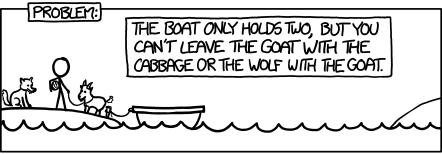
\includegraphics[scale=1]{xkcd/logic_boat_problem}}
		\only<2|handout:2>{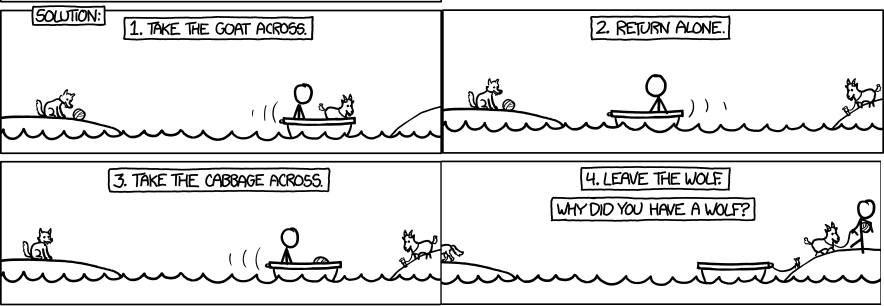
\includegraphics[scale=0.35]{xkcd/logic_boat_sol}}
		\vspace{-7pt}
		\caption{ \texttt{\url{http://xkcd.com/1134/}} }
	\end{figure} 
}

\section{Aussagenlogik}

\begin{frame}
	\frametitle{Aussagenlogik}
	Aussagen sind Sätze, die entweder wahr oder falsch sind.\\
	Der Wahrheitswert muss dabei nicht unbedingt bekannt oder \enquote{tatsächlich ermittelbar} sein.
	
	\pause
	\begin{Beispiel}
		\begin{itemize}
			\item $ 1 + 1 = 2 $ ist eine Aussage. Sie ist wahr.
			\item \enquote{Es gibt nur endlich viele Primzahlen.} ist eine Aussage. Sie ist falsch.
			\pause
			\item Die Goldbachsche Vermutung ist eine Aussage. Ihr Wahrheitswert ist unbekannt.
			\pause
			\item Die Welt wird am 11.11.11111 untergehen ist auch eine Aussage. Wir werden ihren Wahrheitswert aber wohl niemals ermitteln können.
			\pause
			\item \enquote{Gelb} ist keine Aussage.
			\pause
			\item \enquote{Dieser Satz ist falsch.} ist keine Aussage. Dem Satz kann offensichtlich kein Wahrheitswert zugeordnet werden.
		\end{itemize}
	\end{Beispiel}
\end{frame}

\begin{frame}
	\frametitle{Zwei Grundsätze der Aussagenlogik}
	
	\begin{itemize}
		\pause
		\item Jede Aussage ist entweder falsch oder wahr.\\
		Wir schreiben im Folgenden $\BB= \{\text{w}, \text{f}\}$
		\pause
		\item Der Wahrheitswert einer zusammengesetzten Aussage ist durch die
		Wahrheitswerte der Teilaussagen eindeutig festgelegt. \\
		\enquote{$2 + 2 = 5 \; \bimp \; \text{Pinguine können fliegen}$} ist \textbf{wahr}.\\[0.2em]
		%TODO
		%Ex falso quodlibet
	\end{itemize}

	Wir abstrahieren daher vom Inhalt und betrachten \textbf{Aussagevariablen}.
\end{frame}

\begin{frame}
	\frametitle{Syntax}
	\begin{Definition}
		$Var_{AL}$ ist die Menge aller Aussagevariablen. \\
		$A_{AL} = \{ \bleftBr, \brightBr, \bnot, \bund, \boder, \bimp \} \cup Var_{AL}$
	\end{Definition}
	\pause
	\begin{Definition}
		$For_{AL}$ ist die Menge aller syntaktisch korrekten Formeln über $Var_{AL}$.\\
		Formal wird diese induktiv über Konstruktionsabbildungen definiert (\emph{VL}).
		Wendet man Klammereinsparungen an, entspricht das Ergebnis unserer intuitiven Verwendung.
	\end{Definition}
	\pause
	\begin{Beispiel}
		$$Var_{AL} = \{A, B, C\}$$
		$$For_{AL} = \{(A  \bimp B) \boder \bnot B, ...\}$$
	\end{Beispiel}
\end{frame}

\begin{frame}
	\frametitle{Semantik}
	Die Semantik einer aussagenlogischen Formel wird durch Auswertung bestimmt.\\
	Hierbei werden den Symbolen aus $A_{AL}$ boolsche Funktionen zugeordnet.
	
	\pause
	\begin{Definition}
		Eine \textbf{boolesche Funktion} ist eine Abbildung der Form
		$f: \BB^n \to \BB$.
	\end{Definition}

	\pause
	\begin{Beispiel}
		\enquote{Übliche} boolesche Funktionen sind  $b_{\bnot}$,
		$b_{\bund}$, $b_{\boder}$ und $b_{\bimp}$
	\end{Beispiel}
\end{frame}

\begin{frame}<handout:0>
	\frametitle{Semantik}
	\begin{center}
		\begin{huge}
			$$\only<1-2>{\boder}\only<3-4>{\bund}\only<5-6>{\bnot}\only<7-8>{\bimp}$$
		\end{huge}
		Wahrheitstabelle:
		\begin{table}
			\begin{tabular}{|c|c|c|}
				\hline 
				$A$ & \only<1-4,7-8>{$B$} & $\only<1-2>{A \boder B}\only<3-4>{A \bund B}\only<5-6>{\bnot A}\only<7-8>{A \bimp B}$ \\ \hline
				w & \only<1-4,7-8>{w} & \only<2>{w}\only<4>{w}\only<6>{f}\only<8>{w} \\ \hline
				w & \only<1-4,7-8>{f} & \only<2>{w}\only<4>{f}\only<6>{f}\only<8>{f} \\ \hline
				f & \only<1-4,7-8>{w} & \only<2>{w}\only<4>{f}\only<6>{w}\only<8>{w} \\ \hline
				f & \only<1-4,7-8>{f} & \only<2>{f}\only<4>{f}\only<6>{w}\only<8>{w} \\ \hline
			\end{tabular}
		\end{table}
	\end{center}
\end{frame}

\begin{frame}
	\frametitle{Semantik}
	Der Wahrheitswert einer zusammengesetzten Aussage hängt von den Wahrheitswerten der verwendeten Aussagevariablen ab. \\
	\begin{Definition}
		Sei $V \subseteq Var_{AL}$ die Menge der verwendeten Aussagevariablen.\\
		Eine Funktion $I: V \to \BB$ bezeichnet man als \textbf{Interpretation}.
	\end{Definition}
	
	\pause
	
	\begin{Definition}
		Eine \textbf{Tautologie} ist eine aussagenlogische Formel, bei der für alle möglichen Interpretationen $I$ gilt: $val_I(A) = \textbf{w}$.\\[0.5em]
		
		\pause
		Liefert die Auswertung von zwei aussagenlogischen Formeln $A$ und $B$ für jede Interpretation $I$ jeweils den gleichen Wert, also $val_I(A) = val_I(B)$, so bezeichnen wir diese Formeln als \textbf{äquivalent} und schreiben $A \equiv B$.
	\end{Definition}

\end{frame}

\begin{frame}
	\frametitle{Auswertung}
	Für die Auswertung einer Aussagenlogsichen Formel $A$ unter Interpretation $I$ definieren wir die Abbildung $val_I(A)$.\\
	Die Auswertung erfolgt dabei schrittweise.
	
	\begin{align*}
	&val_I((A \bimp B) \boder \bnot B)  \\
	\visible<2->{= \;&b_{\boder} (val_I(A\bimp B), val_I(\bnot B)) \\}
	\visible<3->{= \;&b_{\boder} (b_{\bimp} (val_I(A), val_I(B)), b_{\bnot}(val_I(B))) \\}
	\visible<4->{= \;&b_{\boder} (b_{\bimp} (I(A), I(B)), b_{\bnot}(I(B))) \\}
	\end{align*}
\end{frame}

% TODO
\begin{frame}
	\frametitle{Auswertung}
	\only<1|handout:1>{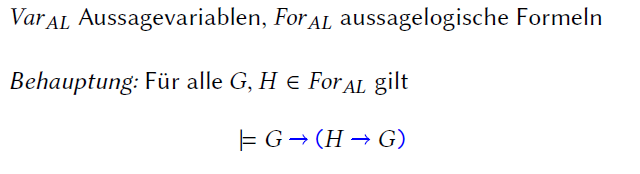
\includegraphics[scale=0.65]{al_uebung_1}\\[2em]
	Quelle: GBI-Übung 2015/2016}
	\only<2|handout:2>{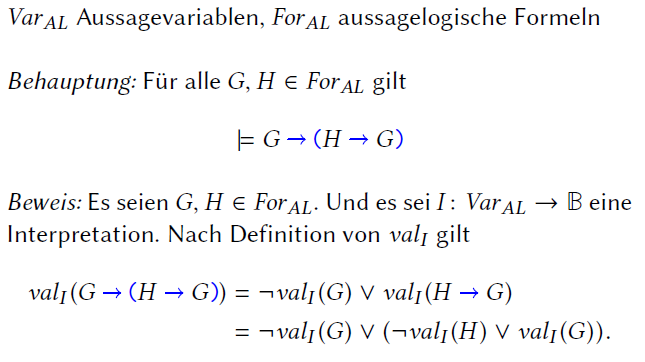
\includegraphics[scale=0.65]{al_uebung_2}}
	\only<3|handout:3>{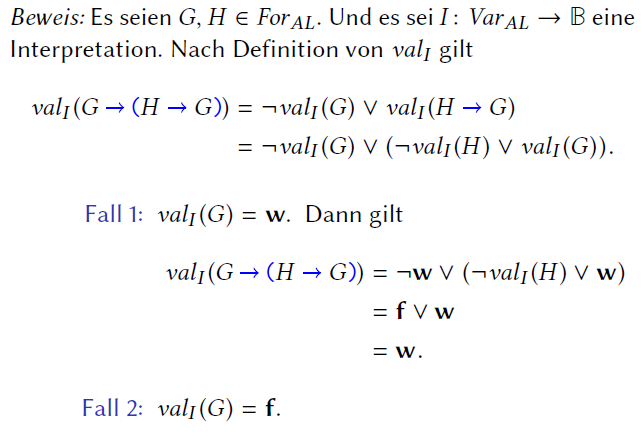
\includegraphics[scale=0.65]{al_uebung_3}}
	\only<4|handout:4>{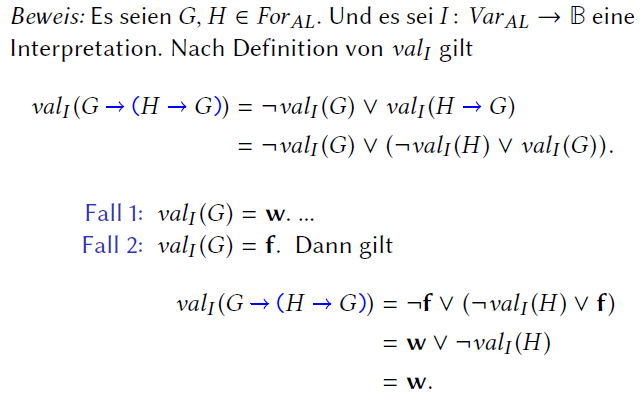
\includegraphics[scale=0.65]{al_uebung_4}}
	\only<5|handout:5>{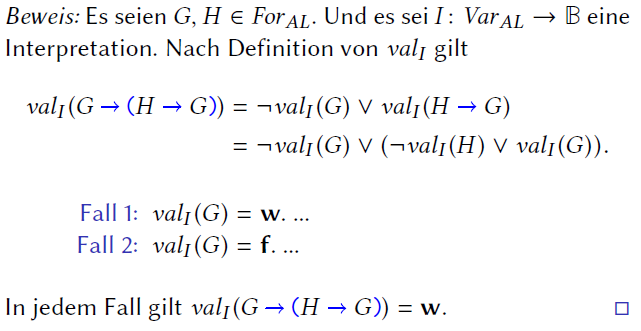
\includegraphics[scale=0.65]{al_uebung_5}}
\end{frame}

\begin{frame}
	\frametitle{Semantik}
	
	Möchte man eine AL-Formel für alle möglichen Interpretationen auswerten, so macht man dies meist in Form einer \textbf{Wahrheitstabelle}.
	
	\begin{block}{Aufgabe}
		Gegeben seien die Formeln
		$$ F_1 = (((B \bimp A) \boder B) \bimp (\bnot A)) \bund B$$
		und
		$$F_2 = \bnot A \bund B$$
		Stellen Sie die Wahrheitstabellen von $F_1$ und $F_2$ auf. Sind die beiden Formeln äquivalent?
	\end{block}
\end{frame}

\begin{frame}
	\frametitle{Lösung}
	Für die Formel $F_1$:
	\begin{table}[H]
	\centering
	\begin{tabular}{|*{6}{c|}}
	\hline
	$A$ & $B$ & $B \bimp A$ &  $\dots \boder B$ & $\dots \bimp \bnot A$ & $\dots \bund B$ \pause \\ \hline
	w & w & w & w & f & f \pause \\ \hline 
	w & f & w & w & f & f \pause \\ \hline
	f & w & f & w & w & w \pause \\ \hline
	f & f & w & w & w & f \\ \hline
	\end{tabular}
	\end{table}
\end{frame}

\begin{frame}
	\frametitle{Lösung}
	Für die Formel $F_2$:
	\begin{table}[h!]
	\centering
	\begin{tabular}{|*{3}{c|}}
	\hline
	$A$ & $B$ & $\bnot A \bund B$ \pause  \\ \hline
	w & w & f \pause  \\ \hline
	w & f & f \pause  \\ \hline
	f & w & w \pause  \\ \hline
	f & f & f \\ \hline
	\end{tabular}
	\end{table}
	Also sind die beiden Formeln äquivalent $$F_1 \equiv F_2$$
\end{frame}

\begin{frame}
	\frametitle{Beweisbarkeit}
	Kalkül, Axiome, Schlussregeln, Modus Ponens, ...\\
	Siehe VL!
\end{frame}

%\input{../Bloecke/VollstaendigeInduktion.tex}

\section{Formale Sprachen}

\begin{frame}
	\frametitle{Rückblick}
	Sei $\Sigma = \{A, B, ..., Z, a, b, ..., z\}$ ein Alphabet.\\
	\pause
	Dann enthält $\Sigma^*$ alle Wörter, die man mit Zeichen aus $\Sigma$ bilden kann. Aber nicht jedes dieser Wörter ist auch sinnvoll.\\[1em]
	
	\enquote{egnarts si efiL} ist kein sinnvolles Wort. \pause Oder? \\[1em]
	\pause
	Wie wir sehen, hängt es immer vom Kontext ab, welche Wörter wir als (syntaktisch) korrekt betrachten.\\
	
\end{frame}

\begin{frame}
	\frametitle{Formale Sprachen}
		\begin{Definition}
			Sei $\Sigma$ ein Alphabet.\\
			Eine formale Sprache $L$ ist eine Teilmenge von $\Sigma^*$.
		\end{Definition}
		\pause
		\vspace{10pt}
		Durch die formale Sprache geben wir an, welche der möglichen Wörter wir als  \emph{syntaktisch korrekt} ansehen.\\
		\pause
		Formale Sprachen werden häufig nicht direkt, sondern über Bildungsvorschriften angegeben.
		
		\pause
		\begin{Beispiel}
			$\Sigma = \{0, 1\}$ \\
			$L = \{ \omega \in \Sigma^* \mid \omega \text{ endet auf } 10 \}  = \{10, 010, 110, 0010, ...\}$
		\end{Beispiel}
\end{frame}

\begin{frame}
	\frametitle{Formale Sprachen}
	
	\begin{Beispiel}
		Formale Sprache $L$ aller Wörter über $A=\{\literal{a},\literal{b}\}$, in denen nirgends das Teilwort $\literal{ab}$ vorkommt.
		\begin{itemize}
			\pause
			\item $L=\{\literal{a},\literal{b}\}^*
			\setminus \{w_1 \cdot \literal{ab} \cdot w_2 \mid w_1,w_2\in
			\{\literal{a},\literal{b}\}^*\}$
			
			\pause
			\item Erst ein beliebiges Wort (evtl. $\varepsilon$) nur aus $\literal{b}$,\\
			danach ein beliebiges Wort (evtl. $\varepsilon$) nur aus $\literal{a}$.
			
			\pause
			\item $L=\{w_1w_2 \mid w_1\in 
			\{\literal{b}\}^*  \text{ und }  w_2\in \{\literal{a}\}^* \}$
		\end{itemize}
	\end{Beispiel}

	\begin{block}{Bemerkungen}
		\begin{itemize}
			\pause
			\item Die Beschreibung einer formalen Sprache ist nicht eindeutig (siehe oben).
			\pause
			\item Immer auf den Unterschied achten: $\{\literal{abc} \} \neq \literal{abc} $
		\end{itemize}
	\end{block}
\end{frame}


\begin{frame}
	\frametitle{Beispiele aus dem Leben}
	\begin{itemize}
		\item Sprache der korrekten IP4-Adressen \pause
		\begin{align*}
		192.168.178.1,\\
		76.147.112.6, ...
		\end{align*} 
		\pause Aber nicht: $000.999.123.666$ \pause
		\item Formale Sprache der Schlüsselwörter in Java $$L = \{ class, int , if, \dots \}$$ \pause
		\item Formale Sprache der legalen Zahlen vom Typ \textbf{int}: Mit $A = \{0...9\}$ 
		\pause $$A \cdot A^* = \{-19, 12849, 1001, 42, ...\}$$ 
		\pause Und minus? Also besser $ \{ -, \varepsilon \} \cdot A \cdot A^*$
	\end{itemize}
\end{frame}


\begin{frame}
	\frametitle{Produkt}
		\begin{Definition}
			Seien $L_1$ und $L_2$ zwei formale Sprachen. Dann bezeichnet
				$$L_1 \cdot L_2 = \{w_1 w_2 \mid w_1 \in L_1 \text{ und } w_2 \in L_2 \}$$
				das \textbf{Produkt} der Sprachen $L_1$ und $L_2$.
		\end{Definition}
		\pause
		In $L_1 \cdot L_2$ sind also alle Wörter enthalten, deren erster Teil aus $L_1$ und deren zweiter Teil aus $L_2$ ist.
	
\end{frame}

\begin{frame}
	\frametitle{Produkt}
	\begin{Beispiele}
		$\{a, b\} \cdot \{c, d\} = \{ac, ad, bc, bd\}$\\[0.3em]
		\pause
		$ L = \{w_1w_2 \mid w_1\in \{\literal{b}\}^* ,  w_2\in \{\literal{a}\}^* \} 
		= \{\literal{b}\}^* \cdot \{\literal{a}\}^* $\\[1em]
		\pause
		Für alle formalen Sprachen $L$ gilt:\\
		$$ L \cdot \{\varepsilon\} = L  \qquad L \cdot \emptyset = \emptyset$$
	\end{Beispiele}
\end{frame}

\begin{frame}
	\frametitle{Potenzen}
	\begin{Definition}
	Damit kann man induktiv die Potenz formaler Sprachen definieren:
	$$L^0 = \{\varepsilon \}$$
	$$L^{i+1} = L^i \cdot L$$
	\end{Definition} \pause
	$L^i$ enthält also alle Kombinationen von $i$ (nicht unbedingt verschiedenen) Wörtern aus $L$.
\end{frame}

\begin{frame}
	\frametitle{Konkatenationsabschluss}
	\begin{Definition}
		Der Konkatenationsabschluss einer formalen Sprache $L$ ist $$L^\ast = \bigcup \limits_{i=0}^\infty L^i$$ 
		\pause
		Der $\varepsilon$-freie Konkatenationsabschluss ist $$L^+ = \bigcup \limits_{i=1}^\infty L^i$$
	\end{Definition} \pause
	Achtung: Der $\varepsilon$-freie Konkatenationsabschluss muss nicht $\varepsilon$-frei sein! \pause
	
	$$ \{\}^* = \{\varepsilon\} $$
\end{frame}


\begin{frame}
	\frametitle{Aufgabe \stars{3}}
	Es sei $A = \{a, b\}$. Beschreiben Sie die folgenden formalen Sprachen mit den Symbolen $\{, \}, a, b,
\varepsilon, \cup, \ast,$ Komma,$ ), ($ und $+$:
	\begin{itemize}
		\item die Menge aller Wörter über $A$, die das Teilwort \code{ab} enthalten.
		\item die Menge aller Wörter über $A$, deren vorletztes Zeichen ein b ist.
		\item die Menge aller Wörter über $A$, in denen nirgends zwei b’s unmittelbar hintereinander vorkommen.
	\end{itemize}
\end{frame}

\begin{frame}
	\frametitle{Lösung}
	\begin{itemize}
		\item \textit{die Menge aller Wörter über $A$, die das Teilwort \code{ab} enthalten.}  \pause
			$$\{a,b\}^\ast \cdot \{ab\} \cdot \{a,b\}^\ast$$ \pause
		\item \textit{die Menge aller Wörter über $A$, deren vorletztes Zeichen ein b ist.}  \pause
			$$\{a,b\}^\ast \cdot \{b\} \cdot \{a,b\}$$ \pause
		\item \textit{die Menge aller Wörter über $A$, in denen nirgends zwei b’s unmittelbar hintereinander vorkommen.}  \pause
			$$\{a, ba\}^\ast \cdot \{b, \varepsilon \}$$
	\end{itemize}
\end{frame}



%\input{../Bloecke/BinäreOperationen.tex}

\begin{frame}	
	\begin{block}{Was ihr nun wissen solltet}
		\begin{itemize}
			\item Aussagenlogik: Syntax und Semantik
			\item Was eine formale Sprache ist und warum das Konzept wichtig ist
			\item Wie man einfache formale Sprachen formal angeben kann
			\item Einfache Operationen auf formalen Sprachen
		\end{itemize}
	\end{block}
	
	\begin{block}{Was nächstes Mal kommt}
		\begin{itemize}
			\item So viele Sprachen: Mehr zu formalen Sprachen
			\item Aus 2 mach 10: Übersetzungen
		\end{itemize}
	\end{block}
\end{frame}

%% Letzte Seite
\lastframe{0.45}{0}{xkcd/logic_drivers.png}{https://xkcd.com/589/}
\slideThanks

\end{document}
